\chapter{Sounds of the General American English}
\label{ch:english_language}
In the \textit{General American English} there are 41 different sounds in which can be structured by the way they are produced. In \ref{table:english_sounds} is shown the kind of sounds with the respective number of possible productions. Each type will be described into a dedicated section of this thesis. An important factor is the way of how the \textit{constriction} of the flow of air is made. In fact, to distiguish between \textit{consonants}, \textit{semivowels} and \textit{vowels}, the \textit{degree} of constriction is checked. Instead, for \textit{sonorant} consonants the air flow is continuous with no pressure. \textit{Nasal} consonants have an occlusive consonant made with a lowered velum allowing the airflow in the nasal cavity \cite{nasal_consonants_wiki}. The \textit{continuant} consonants are produced without blocking the airflow in the oral cavity.

\begin{table}[h]
    \centering
    \begin{tabular}{|c|c|}
        \hline
        \textbf{Type}& \textbf{Number} \\ \hline
        Vowels     & 18     \\ \hline
        Fricatives & 8      \\ \hline
        Stops      & 6      \\ \hline
        Nasals     & 3      \\ \hline
        Semivowels & 4      \\ \hline
        Affricates & 2      \\ \hline
        Aspirant   & 1      \\ \hline
    \end{tabular}
    \caption {Type of English sounds}
\label{table:english_sounds}
\end{table}

%%%%%%%%%%%%%%%%%%%%%%%%%%%%%%%%%%%%%%%%%%%%%%%%%%%%%%%%%%%%%%%%%%%%%%%%%%%%%%%%%%%%%%%%%%%%%%%%%%%%%%%%%%%%%%%%%%%%%%%%%%%%%%%%%%

\section{Vowel production}
\label{sec:vowel_production}
Generally speaking, when a vowel is pronunced, there is no air-constriction in the flow. This means that the ariculators like the tongue, lips and the uvula do not touch allowing the flow of air from the lungs. The consonants instead have another pattern when producing them. Moreover, to produce each vowel, the mouth has to make a different shape in such a way that the resonance is different. \ref{fig:vowels_prod} shows the way the mouth, the jaw and the lips are combined in a such a way to produce the acoustinc sound of a vowel.

\begin{figure}[!ht]
    \centering
    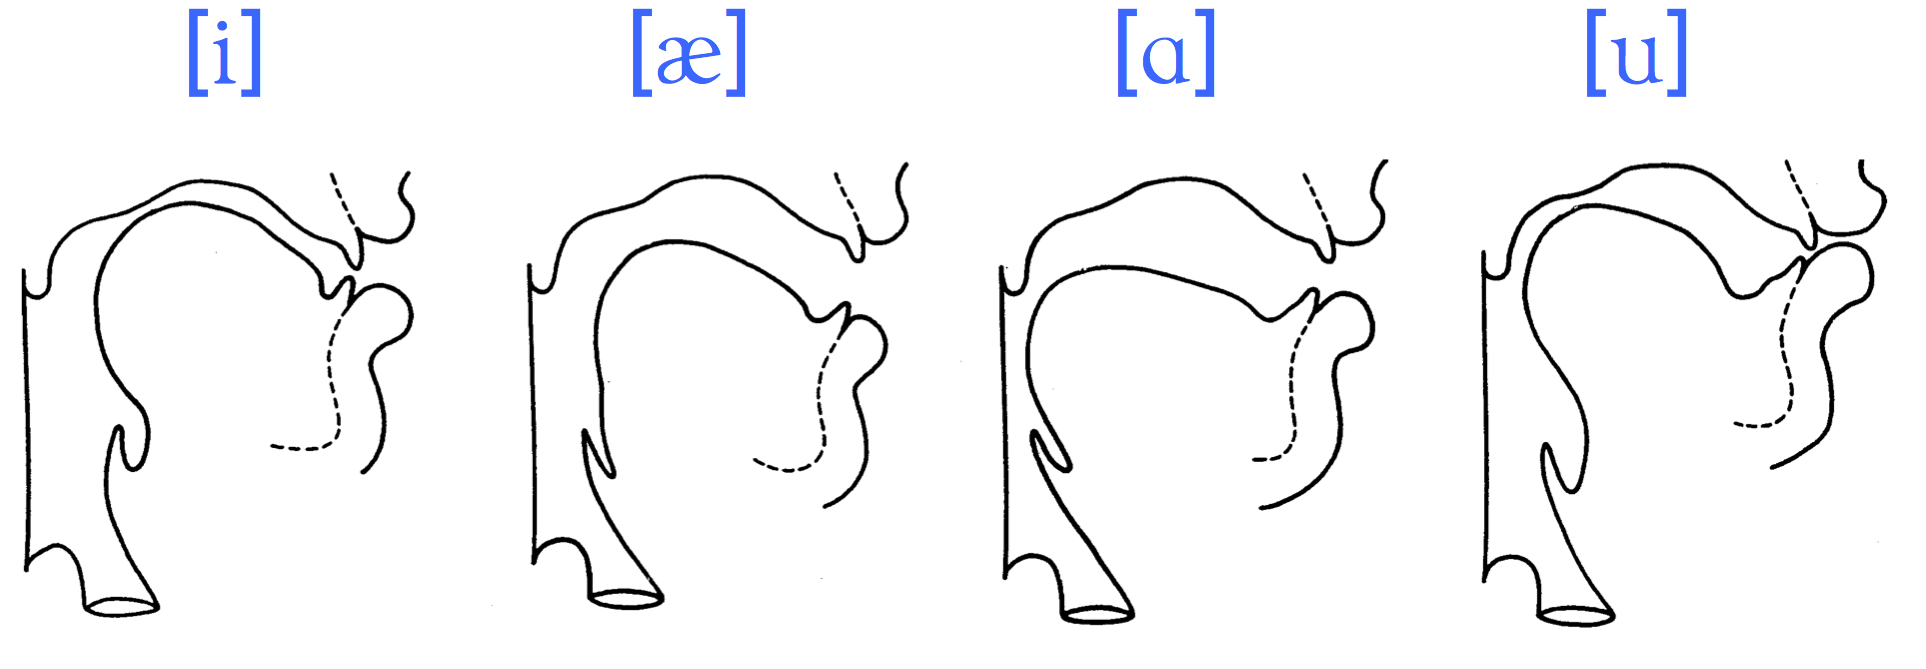
\includegraphics[scale=0.5]{Figures/vowels_prod.png}
    \caption{Vowels production \cite{mit_phonetics}}
    \label{fig:vowels_prod}
\end{figure}

\subsection{Vowel of American English}
\label{sub:vowel_of_american_english}
There are 18 different vowels in American English that can be grouped by three different sets: the \textbf{monopthongs}, the \textbf{diphthongs}, and the \textbf{schwa's} - or reduced vowels.

\begin{figure}[!ht]
    \centering
    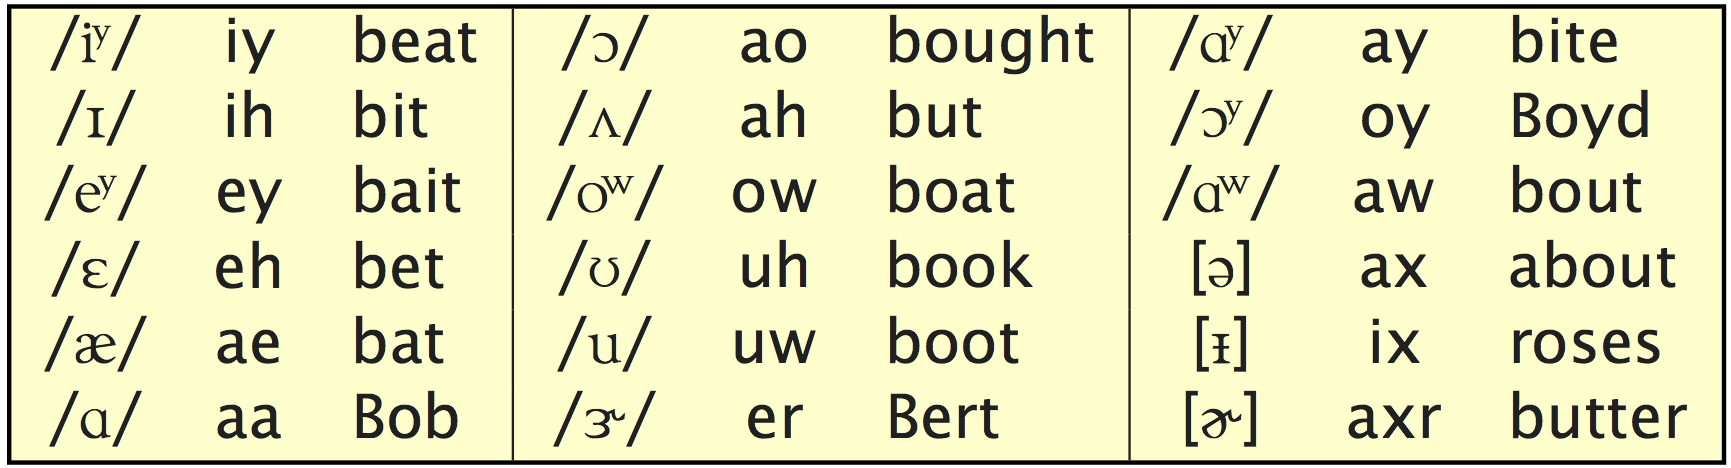
\includegraphics[scale=0.5]{Figures/vowels_sets.png}
    \caption{Example of words depending on the group \cite{mit_phonetics}}
    \label{fig:vowels_sets}
\end{figure}

The first column shows some examples of monopthongs. A \textit{monopthong} is a clear vowel sound in which the utterance are fixed at both the beginning and at the end. The central part of the picture represents the dipthongs. A \textit{dipthong} is the sound produced by two vowels when they occur within the same syllable \cite{dipthong_wiki}. In the last column are depictes some examples of reduced vowels. \textit{Schwa's} refers to the vowel sound that stays in the mid-central of the word. In general, in the english language, the schwa is found in unstressed position \cite{schwa_wiki}.

%%%%%%%%%%%%%%%%%%%%%%%%%%%%%%%%%%%%%%%%%%%%%%%%%%%%%%%%%%%%%%%%%%%%%%%%%%%%%%%%%%%%%%%%%%%%%%%%%%%%%%%%%%%%%%%%%%%%%%%%%%%%%%%%%%

\subsection{Formants}
\label{sub:formants}
A \textit{formant} is the resonant frequency of a vocal track that resonate the loudest. In a spectrum graph, formants are represented by the peaks. In \ref{fig:peaks_formants} it is possibile to see how the three first formants are defined by the peaks. The pictures is the \textit{envelope} of a spectogram of the vowel \textbf{[i]}. Frequencies are the most relevant information to determine which vowel has been pronounced. In general, within a spectrum graph there may be a different number of formants, although the most relevant are the first three and they are named \textbf{F1}, \textbf{F2} and \textbf{F3}.

\begin{figure}[!ht]
    \centering
    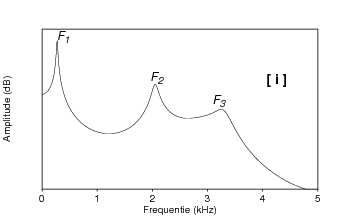
\includegraphics[scale=0.6]{Figures/peaks_formants.png}
    \caption{Spectral envelope of the [i] vowel pronunciation. F1, F2 and F3 are the first 3 formants \cite{formants_peaks}}
    \label{fig:peaks_formants}
\end{figure}

\noindent The frequencies produced by the formants are highly dependent on the tongue position. In fact, formant \textit{F1}'s frequencies are produced when the tongue is either in a \textit{high} or \textit{low} position, whereas formant \textit{F2} whene the tongue is in either \textit{front} or \textit{back} position and formant \textit{F3} when the tongue is doing \textit{Retroflexion}. \textbf{Retroflextion} is more present when pronouncing the consonant \textit{R}

%%%%%%%%%%%%%%%%%%%%%%%%%%%%%%%%%%%%%%%%%%%%%%%%%%%%%%%%%%%%%%%%%%%%%%%%%%%%%%%%%%%%%%%%%%%%%%%%%%%%%%%%%%%%%%%%%%%%%%%%%%%%%%%%%%

\subsection{Vowel duration}
\label{sub:vowel_duration}
The duration of a vowel is the time that taken when pronounicing it. The duration is measured in \textit{centiseconds} and in English\footnote{In Icelandic as well} the different lengths are defined by certain rules. In general, the length of \textit{lax vowels} such as /\textipa{I e \ae 2 6 u 9}/ are short whereas \textit{tense vowels} like /\textipa{i: A: O: u: 3:}/ including dipthongs /\textipa{eI aI OI 9U aU I9 ea U9}/ have a variable lentgh but longer than lax vowels \cite{vowel_length}. In \ref{fig:vowel_length} is shown an example of time-length of some vowels.
\noindent In General American English, the length of vowels are not as distinctive as in the \textit{RP}\footnote{More commonly referred as the Standard English in the UK} pronunciation. In some American accents, to express an emphasis the length of vowels can be extended.

\begin{figure}[!ht]
    \centering
    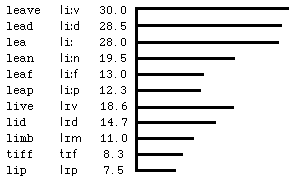
\includegraphics[scale=0.6]{Figures/vowel_length.png}
    \caption{RP vowel length \cite{vowel_length}}
    \label{fig:vowel_length}
\end{figure}

%%%%%%%%%%%%%%%%%%%%%%%%%%%%%%%%%%%%%%%%%%%%%%%%%%%%%%%%%%%%%%%%%%%%%%%%%%%%%%%%%%%%%%%%%%%%%%%%%%%%%%%%%%%%%%%%%%%%%%%%%%%%%%%%%%

\section{Fricative Production}
\label{sec:fricative_production}
A \textbf{fricative} is a consonant sound that is produced by narrowing the cavity causing a friction as the air goes through it \cite{fricatives}. There are eight fricatives in American English divided in two categories: \textit{Unvoiced} and \textit{Voiced}. These two categories are often called \textit{Non-Strident} and \textit{Strident} that means that there is a constriction behind the alveolar ridge.

\begin{figure}[!ht]
    \centering
    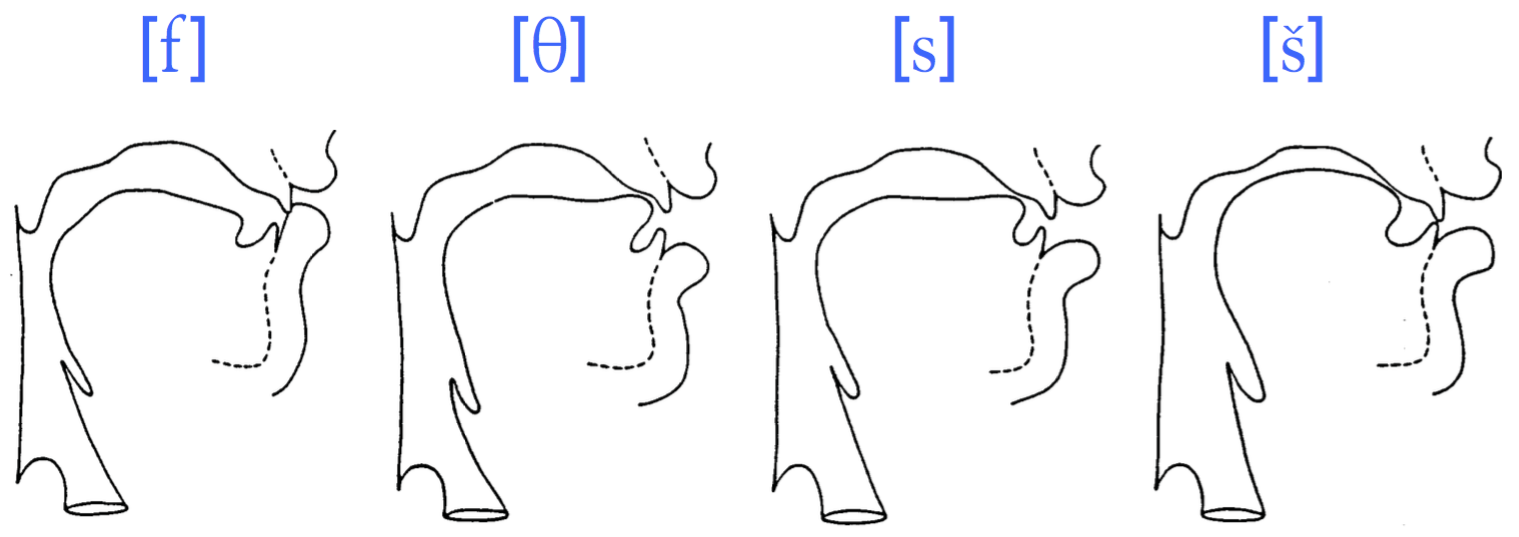
\includegraphics[scale=0.5]{Figures/fricative_production.png}
    \caption{Fricative production \cite{mit_phonetics}}
    \label{fig:fricative_prod}
\end{figure}

\noindent In \ref{fig:fricative_ex} it is possible to see some examples of these two categories. Each consonant also belongs to a specific articulation position. In fact, each figure in \ref{fig:fricative_prod} represents a specific articulation position. From left to right we have: \textit{Labio-Dental} (Labial), \textit{Interdental} (Dental), \textit{Alveolar} and \textit{Palato-Alveolar} (Palatal).

\begin{figure}[!ht]
    \centering
    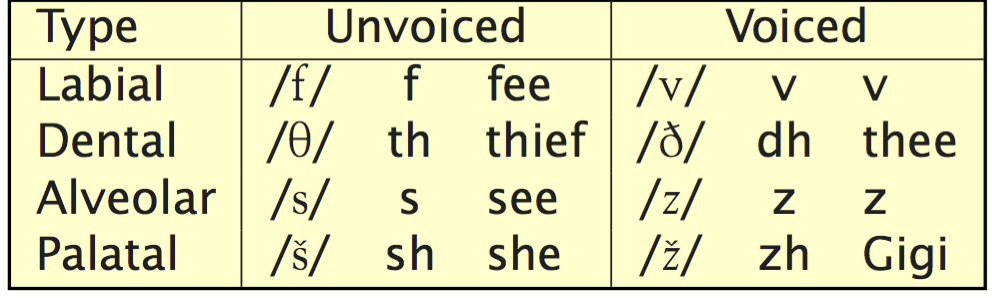
\includegraphics[scale=0.5]{Figures/fricative_examples.png}
    \caption{Fricative examples of productions \cite{mit_phonetics}}
    \label{fig:fricative_ex}
\end{figure}

%%%%%%%%%%%%%%%%%%%%%%%%%%%%%%%%%%%%%%%%%%%%%%%%%%%%%%%%%%%%%%%%%%%%%%%%%%%%%%%%%%%%%%%%%%%%%%%%%%%%%%%%%%%%%%%%%%%%%%%%%%%%%%%%%%

\section{Affricate Production}
\label{sec:Affricate Production}
An \textbf{affricate} consonant is produced by stopping the airflow first and then release it similar to a fricative. The result is also considered a \textit{turbolence noise} since the produced sound has a suddent release of the constriction. In English there only two affricate phonemes, as depicted in \ref{fig:affricate_prod}.

\begin{figure}[!ht]
    \centering
    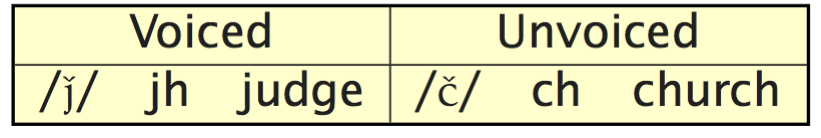
\includegraphics[scale=0.5]{Figures/affricative_production.png}
    \caption{Affricative production \cite{mit_phonetics}}
    \label{fig:affricate_prod}
\end{figure}

%%%%%%%%%%%%%%%%%%%%%%%%%%%%%%%%%%%%%%%%%%%%%%%%%%%%%%%%%%%%%%%%%%%%%%%%%%%%%%%%%%%%%%%%%%%%%%%%%%%%%%%%%%%%%%%%%%%%%%%%%%%%%%%%%%

\section{Aspirant Production}
\label{sec:Aspirant Production}
An \textbf{aspirant} consonant is a strong outbreak of breath produced by generating a turbolent airflow at glottis level. In American English exists only one aspirant consonant and it is the /\textipa{h}/, for instance in the word \textit{hat}.

%%%%%%%%%%%%%%%%%%%%%%%%%%%%%%%%%%%%%%%%%%%%%%%%%%%%%%%%%%%%%%%%%%%%%%%%%%%%%%%%%%%%%%%%%%%%%%%%%%%%%%%%%%%%%%%%%%%%%%%%%%%%%%%%%%

\section{Stop Production}
\label{sec:Stop Producton}
A \textbf{Stop} is a consonant sound in which the oral cavity is blocked in such a way that the airflow ceases. The stop consonant is also known as \textit{plosive} which means that it is an oral \textit{occlusive} sound \cite{stop_consonants_wiki}. The occlusion can come up in three different variance as shown in \ref{fig:stop_prod}: from left to right we have a \textit{Labial} occlusion, the \textit{Alveolar} occlusion and the \textit{Velar} occlusion. The pressure built up in the vocal tract, determine the produced sound depending on which occlusion is performed.

\begin{figure}[!ht]
    \centering
    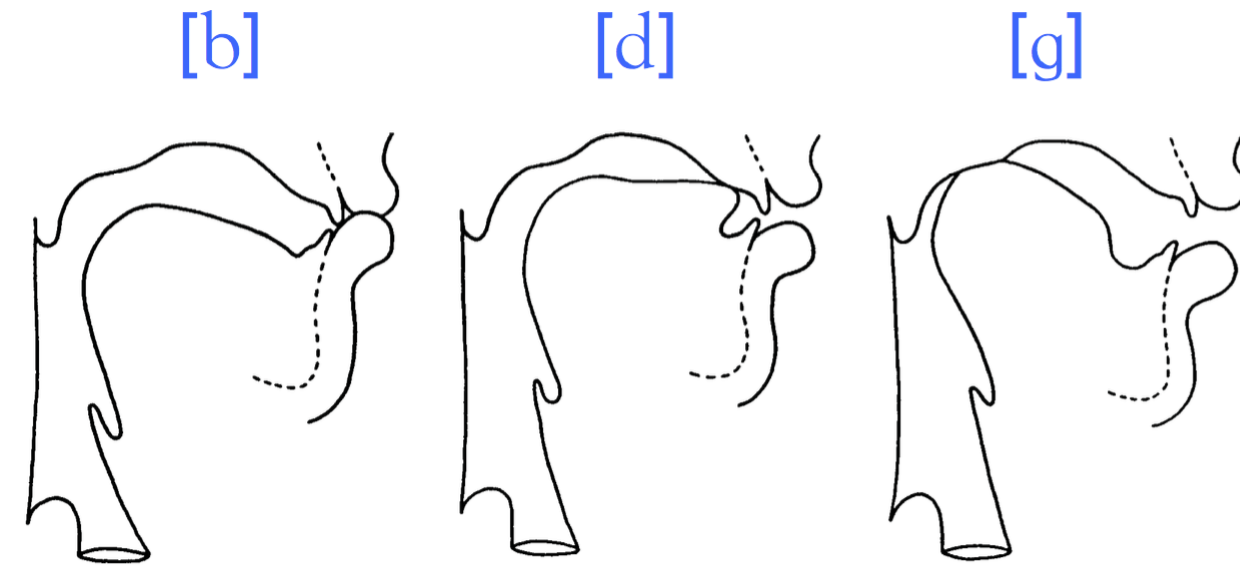
\includegraphics[scale=0.5]{Figures/stop_production.png}
    \caption{Stop production \cite{mit_phonetics}}
    \label{fig:stop_prod}
\end{figure}

\noindent In American English there are six stop consonants, as represented in \ref{fig:stop_ex}. As for the fricative consonants, the two main categories are the \textit{Voiced} and \textit{Unvoiced} sounds. Although, a particularity of the Unvoiced stops is that they are typically \textit{aspirated} whereas in the Voiced ones there is a \textit{voice-bar} during the closure movement. These two particularities are very useful where analyzing the formants because the frequencies are very well distinguished allowing a classification system to better understand the difference between stop phonemes.

\begin{figure}[!ht]
    \centering
    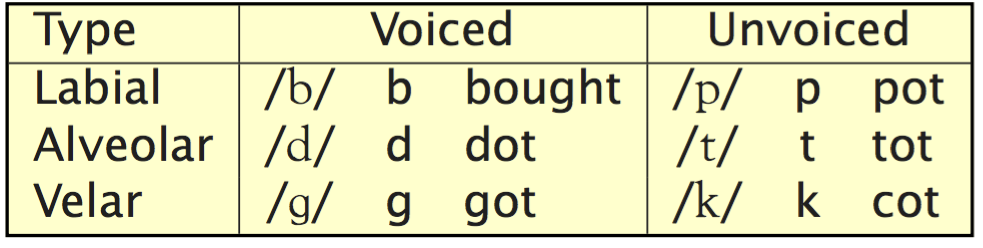
\includegraphics[scale=0.5]{Figures/stop_examples.png}
    \caption{Stop examples of production \cite{mit_phonetics}}
    \label{fig:stop_ex}
\end{figure}

%%%%%%%%%%%%%%%%%%%%%%%%%%%%%%%%%%%%%%%%%%%%%%%%%%%%%%%%%%%%%%%%%%%%%%%%%%%%%%%%%%%%%%%%%%%%%%%%%%%%%%%%%%%%%%%%%%%%%%%%%%%%%%%%%%

\section{Nasal Production}
\label{sec:Nasal Production}
A \textbf{Nasal} is a occlusive consonant sound that is produced with a \textit{lowered velum}, allowing the airflow to go out through the nostrils \cite{nasal_consonants_wiki}. Becuase the airflow escapes through the nose, the consonants are produced with a closure in the vocal tract. \ref{fig:nasal_prod} shows the three different positions to produce a nasal consonant. From left to right we have \textit{Labial}, \textit{Alveolar} and \textit{Velar}. \\
\noindent Due to this particularity, the frequencies of nasal \textit{murmurs} are quite similar. If we take a look on the spectrogram in \ref{fig:nasal_spectrogram}, it is possible to notice that nasal consonants have a high similarity. In a classification system, this can be a problem.

\begin{figure}[!ht]
    \centering
    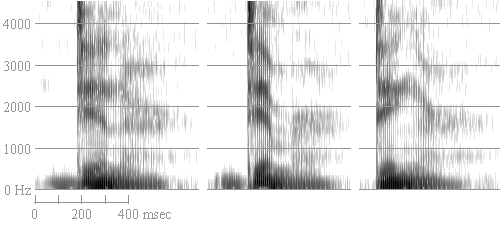
\includegraphics[scale=0.6]{Figures/nasal_spectrogram.png}
    \caption{Nasal Spectrograms of "dinner", "dimmer", "dinger" \cite{nasal_spectrogram}}
    \label{fig:nasal_spectrogram}
\end{figure}

\begin{figure}[!ht]
    \centering
    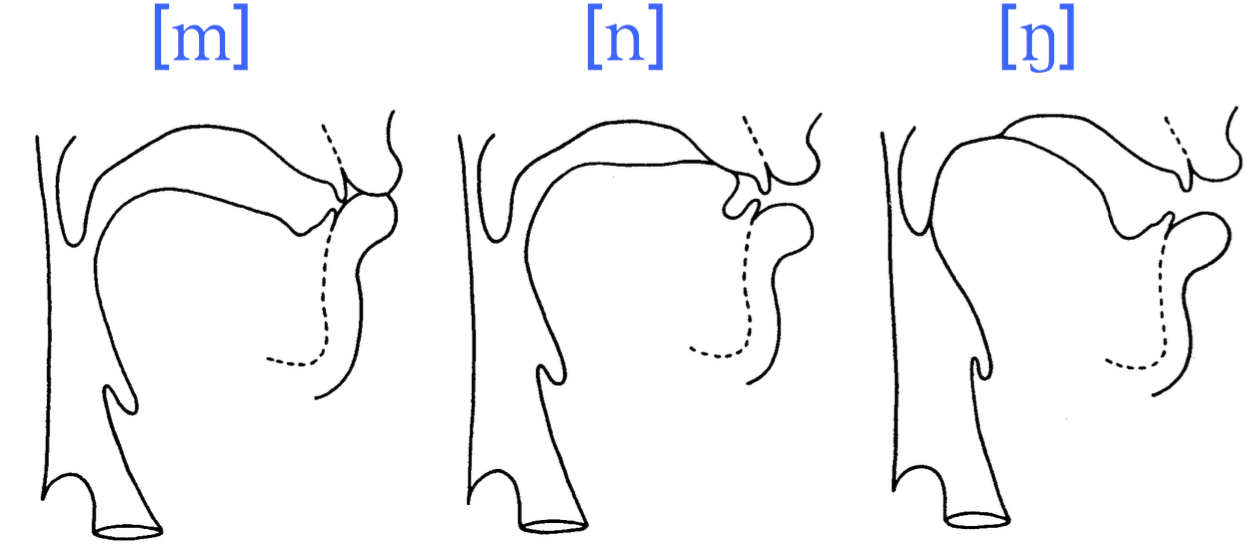
\includegraphics[scale=0.5]{Figures/nasal_production.png}
    \caption{Nasal production \cite{mit_phonetics}}
    \label{fig:nasal_prod}
\end{figure}

\noindent Since the sound produced by a nasal is produced with an occlusive vocal tract, each consonant is \textbf{always attached} to a vowel and it can can form an entire syllable. Although, in English, the consonant /\textbf{\textipa{N}}/ always occur immediately after a vowel. In \ref{fig:nsal_ex} are shown some examples of nasal consonants divided by articulation position.

\begin{figure}[!ht]
    \centering
    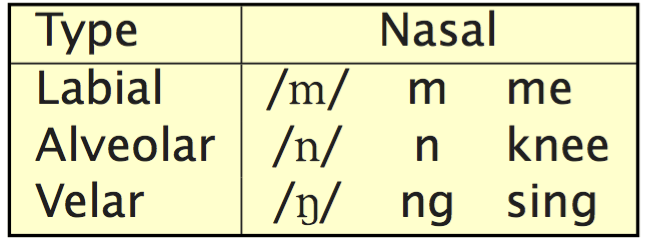
\includegraphics[scale=0.5]{Figures/nasal_examples.png}
    \caption{Nasal examples of production \cite{mit_phonetics}}
    \label{fig:nsal_ex}
\end{figure}

%%%%%%%%%%%%%%%%%%%%%%%%%%%%%%%%%%%%%%%%%%%%%%%%%%%%%%%%%%%%%%%%%%%%%%%%%%%%%%%%%%%%%%%%%%%%%%%%%%%%%%%%%%%%%%%%%%%%%%%%%%%%%%%%%%

\section{Semivowels Production}
\label{sec:Semivowels Production}
A \textbf{semivowel} is a sound that is very close to a vowel sound but it works more likely as a syllable boundary rather than a core of a syllable \cite{ladefoged1998sounds}. A typical example of semivowels in English are the \textbf{y} and \textbf{w} in words \textit{yes} and \textit{west}. In the \textit{IPA} alphabet they are written /\textipa{j}/ and /\textipa{w}/ and they correspond to the vowels /\textipa{i:}/ and /\textipa{u:}/ in the words \textit{seen} and \textit{moon}. In \ref{fig:semivowel_ex} there are some examples of semivowels production. \\
\noindent The sound is produced by making a constriction in the oral cavity without having any sort of air turbolance. To achieve that, the articulation motion is slower than other consonants becuase the laterals\footnote{They are a pair of upper teeth that are located laterally from the central incisors \cite{laterals_wiki}} form a complete closer combined with a tongue tip. In this way the airflow has to pour out using the sides of the constriction.

\begin{figure}[!ht]
    \centering
    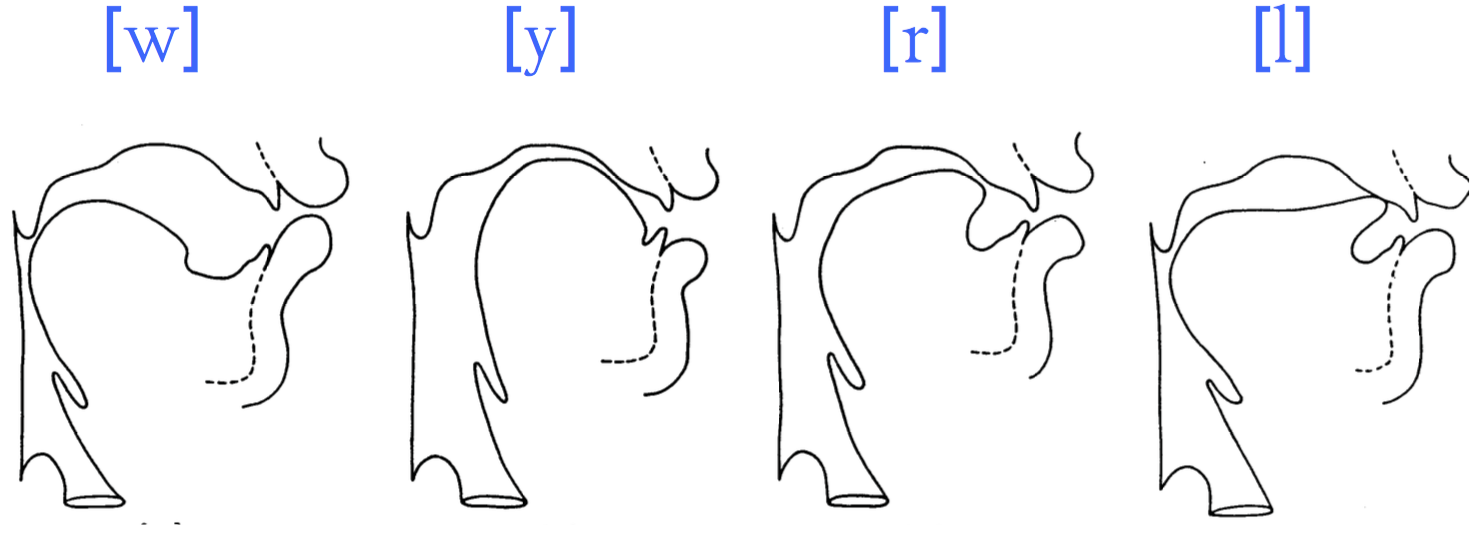
\includegraphics[scale=0.5]{Figures/semivowel_production.png}
    \caption{Semivowel production \cite{mit_phonetics}}
    \label{fig:semivowel_prod}
\end{figure}

\noindent In American English there are four semivowels and they are depiscted in \ref{fig:semivowel_prod}. An important fact of semivowels is that they are always close to a vowel. Although, the /\textipa{l}/ can form an entire syllable by itself when there is no stress in a word.

\begin{figure}[!ht]
    \centering
    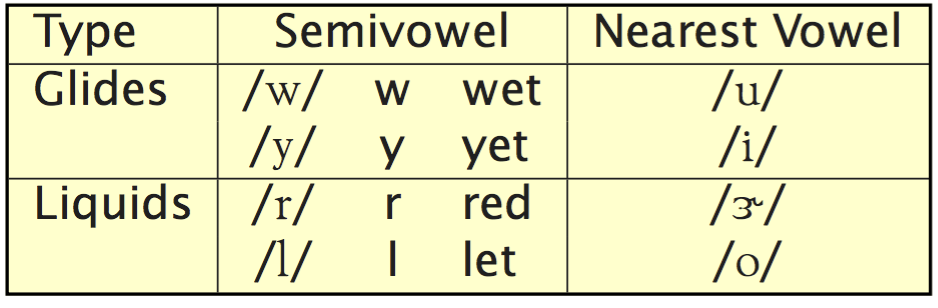
\includegraphics[scale=0.5]{Figures/semivowel_examples.png}
    \caption{Semivowel examples of production \cite{mit_phonetics}}
    \label{fig:semivowel_ex}
\end{figure}

%%%%%%%%%%%%%%%%%%%%%%%%%%%%%%%%%%%%%%%%%%%%%%%%%%%%%%%%%%%%%%%%%%%%%%%%%%%%%%%%%%%%%%%%%%%%%%%%%%%%%%%%%%%%%%%%%%%%%%%%%%%%%%%%%%

\subsubsection{Acousitc Properties of Semivowels}
\label{ssub:Acousitc Properties of Semivowels}
Semivowels have some properties that are taken into account when doing any sort of analysis. In fact, /\textipa{w}/ and /\textipa{l}/ are the semiwovels that are more confusable because both are characterized by a \textit{low} range of frequencies for both formants \textit{F1} and \textit{F2}. Although, the /\textipa{w}/ can be distinguished by the \textit{rapid falloff} in the F2 spectrogram whereas /\textipa{l}/ has more often a \textit{high frequency energy} compared to /\textipa{w}/. The \textbf{energy} is the relationship between the \textit{wavelength} and the \textit{frequency}. So, having a high energy means that there is a high frequency value and a small wavelength \cite{energy_relationship}. \\
\noindent The semivowel /\textipa{y}/ is characterized by having a very low frequency value in formant F1 and a very high in formant F2. The /\textipa{r}/ instead is presented with a very low frequency value of formant F3. \\


%%%%%%%%%%%%%%%%%%%%%%%%%%%%%%%%%%%%%%%%%%%%%%%%%%%%%%%%%%%%%%%%%%%%%%%%%%%%%%%%%%%%%%%%%%%%%%%%%%%%%%%%%%%%%%%%%%%%%%%%%%%%%%%%%%

\section{The Syllable}
\label{sec:The syllable}
The definition of the \textbf{syllable} can be divided in two sub-definition: one from the phonetic point of view and one from the phonological point of view. \\
\noindent In phonetic analysis, the syllable is a basic unit of speech in which they \textit{"are usually described as consisting of a centre which has little or no obstruction to airflow and which sounds comparatively loud; before and after that centre (...) there will be greater obstruction to airflow and/or less loud sound"} \cite{roach2000phonology}. Taking the word \textit{cat} (/\textipa{k\ae t}/) as example, the \textbf{centre} is defined by the vowel /\textipa{\ae}/ in which takes place only a little obstruction. The surronding \textit{plosive} consonants (/\textipa{k}/ and /\textipa{t}/) the airflow is completely blocked \cite{syllable_site}. \\
\noindent A phonological definition of the syllable establishes that it is \textit{"a complex unit made up of nuclear and marginal elements"}\cite{laver1994principles}. In this context, the vowels are considered the \textbf{Nuclear} elements or syllabic segments whereas the \textbf{Marginal} ones are the consonants or non-syllabic segments \cite{syllable_site}. Considering the word \textit{paint} (/\textipa{peInt}/) as example, the nuclear element is defined by the diphtong /\textipa{eI}/ whereas /\textipa{p}/ and /\textipa{nt}/ are the marginal elements.

\subsection{Syllable Structure}
In the phonological theory, the syllable can be decomposed in a hierarchical structure insted of a linear one. The structure starts with the $\sigma$ letter in which represents not only the root, but the syllable itself. Immediately after, there are two \textit{branches} called \textbf{constituents} that they represents the \textit{Onset} and the \textit{Ryhme}. The left branch includes any consonants that precede the vowel (or Nuclear element), whereas the right branch includes both the nuclear element and any consonants (or Marginal elements) that potentially could follow it. \\
\noindent Usually, the ryhme branch is further split in two other branches represented by the \textbf{Nucleus} and the \textbf{Coda}. The first on represent the nuclear element in the syllable. The second one instead, subsumes all the consonants that follow the Nucleus in the syllable \cite{syllable_site}. In \ref{fig:syllable_structure} there is a representation of the syllable structure based on the word \textit{plant}.

\begin{figure}
    \begin{center}
        \fbox{
            \begin{forest}
              for tree={
                parent anchor=south,
                child anchor=north,
                align=center,
                if n children=0{
                  font=\itshape,
                  tier=terminal,
                }{},
              }
              [$\sigma$
                [onset [CC [\textipa{pl}]]]
                [rhyme [Nucleus [V [\textipa{\ae}]]][Coda [C [\textipa{nt}]]]]
              ]
            \end{forest}
        }
    \end{center}
    \caption{Tree structure of the word \textbf{plant}\protect\footnotemark}
    \label{fig:syllable_structure}
\end{figure}

\footnotetext{\textbf{C} means \textit{Consonant} whereas \textbf{V} means \textit{Vowel}}
